\textbf{P1)} \textcolor{red}{[Control 3 - 2025-10]} Una barra de masa $m$ y largo $l$ está articulada sin roce en el punto fijo $O$. Un resorte horizontal de constante de dureza $k$ está conectado al centro de gravedad $G$ de la barra. El resorte está inicialmente en su largo natural cuando la barra está en equilibrio en posición vertical. Se perturba el equilibrio de la barra con un ángulo $\theta_0 = 3^{\circ}$, siendo $\theta$ el ángulo que forma la barra respecto de la vertical, en el sentido de las manecillas del reloj.

\begin{enumerate}[a)]
\item Determine la ecuación diferencial para $\theta$. Pequeñas oscilaciones. (2 ptos.)
\item Determine el valor mínimo de $k$ para que existan pequeñas oscilaciones. (2 ptos.)
\item Considere $m = 1\ \text{kg}$, $l = 0.5\ \text{m}$, $k = 100\ \text{N/m}$ y $g = 9.8\ \text{m/s}^2$. Calcule el período de oscilación de la barra y $\theta(t)$. (2 ptos.)
\end{enumerate}

\vspace{0.3cm}
\begin{center}
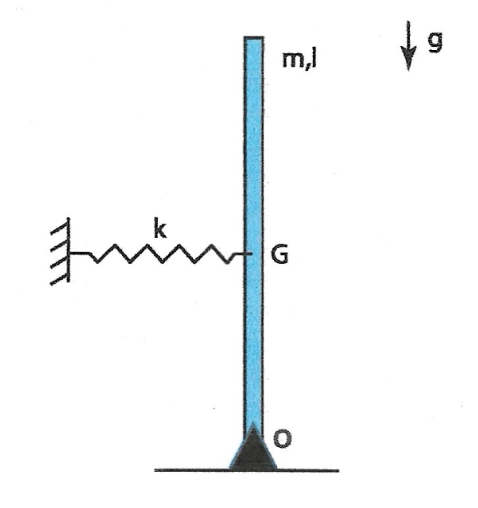
\includegraphics[width=0.32\textwidth]{imagenes/P1a6.PNG}
\end{center}



